\chapter{Аналитический раздел}
В данном разделе будут рассмотрены теоретически основы работы конвейера при применении его к трём алгоритмам: алгоритму поиска максимума, алгоритму поиска минимума, алгоритму поиска суммы всех элементов.

\section{Алгоритм поиска максимума}
Алгоритм поиска максимума будет реализован в виде простейшего алгоритма поиска максимума с перебором всех элементов массива. То есть каждый элемент сравнивается с переменной, хранящей значение локального максимума и если эта переменная больше, чем максимум, то её значение записывается в переменную максимума.

\section{Алгоритм поиска минимума}
Алгоритм поиска минимума будет реализован в виде простейшего алгоритма поиска минимума с перебором всех элементов массива. То есть каждый элемент сравнивается с переменной, хранящей значение локального минимума и если эта переменная больше, чем минимум, то её значение записывается в переменную минимума.

\section{Алгоритм поиска суммы}
Алгоритм поиска минимума будет реализован в виде простейшего алгоритма поиска минимума с перебором всех элементов массива. То есть каждый элемент добавляется к переменной, хранящей значение суммы всех элементов.

\section{Конвейерная обработка данных}
При конвейерной обработке данных используется принцип конвейерного производства, заключающийся в том, что некая крупная задача разделяется на множество коротких операций, которое делается параллельно. Данный способ организации решения каких-либо задач имеет наибольшее преимущество при потоковом решении множества однотипных подзадач, которые разбиваются так, что каждая операция может быть выполнена на одной из стадий конвейера, в результате мы получаем систему, в которой параллельно выполняется сразу несколько подзадач нескольких разных задач. В данной лабораторной работе мы выделили три задачи, которые последовательно обрабатываются на конвейерной ленте.

\section{Вывод}
В данном разделе были рассмотрены основные теоретические сведения об алгоритмах поиска максимума, минимума и суммы элементов в массиве. В результате были сделаны выводы о том, что на вход алгоритму массив целых чисел произвольных размеров, на выходе программа максимум, минимум и сумму всех элементов в массиве. Алгоритмы работают на массивах с размерностями от 0 до физически возможного предела для изпользуемой машины. В качестве критерия для сравнения эффективности алгоритмов будет использоваться время работы на матрицах различного размера. Также была рассмотрена конвейерная обработка данных и сделаны выводы о том, как именно будет организован данный процесс.

\chapter{Конструкторский раздел}

В данном разделе будут рассмотрены схемы, структуры данных, способы тестирования, описания памяти для следующих алгоритмов:
\begin{enumerate}
	\item алгоритм поиска максимума;
	\item алгоритм поиска минимума.
	\item алгоритм поиска суммы всех элементов;
	\item алгоритм решения задачи без конвейера;
	\item алгоритм решения задачи с конвейером.
\end{enumerate}

\section{Тестирование алгоритмов}

Описание классов эквивалентности:
\begin{enumerate}
	\item проверка работы на общем случае.
\end{enumerate}

Описание тестов:
\begin{enumerate}
	\item тест на общем случае - на вход подаётся массив размерама n, возвращаемый результат сравнивается с заранее известным правильным результатом.
\end{enumerate}

\section{Алгоритм поиска максимума}

Используемые типы и структуры данных включают в себя:
\begin{enumerate}
	\item integer, целое число - используется для хранения индексов массива, размера массива;
	\item array, массив целых чисел - используется для хранения серии целых чисел.
\end{enumerate}

\newpage

\begin{figure}[ph!]
	\center{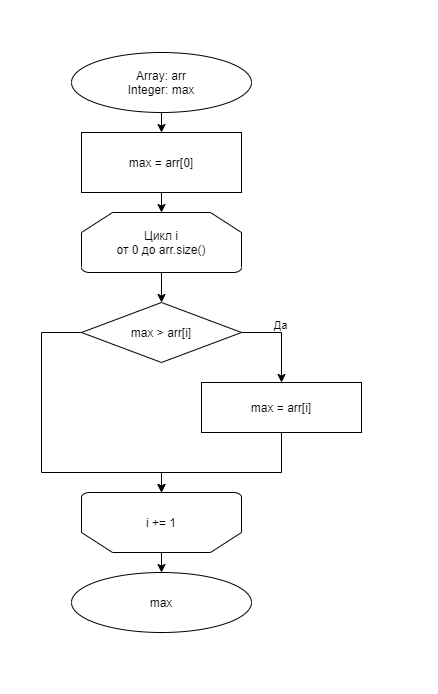
\includegraphics[scale=0.8]{max_scheme}}
	\caption{Схема алгоритма поиска максимума}
\end{figure}

\section{Алгоритм поиска минимума}

Используемые типы и структуры данных включают в себя:
\begin{enumerate}
	\item integer, целое число - используется для хранения индексов массива, размера массива;
	\item array, массив целых чисел - используется для хранения серии целых чисел.
\end{enumerate}

\newpage

\begin{figure}[ph!]
	\center{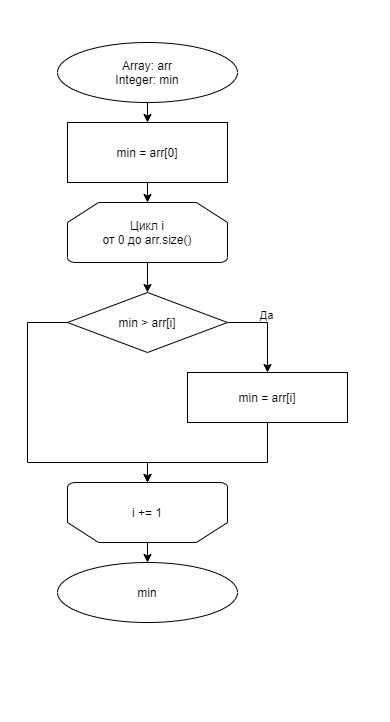
\includegraphics[scale=0.8]{min_scheme}}
	\caption{Схема алгоритма поиска минимума}
\end{figure}

\section{Алгоритм поиска суммы всех элементов}

Используемые типы и структуры данных включают в себя:
\begin{enumerate}
	\item integer, целое число - используется для хранения индексов массива, размера массива;
	\item array, массив целых чисел - используется для хранения серии целых чисел.
\end{enumerate}

\newpage

\begin{figure}[ph!]
	\center{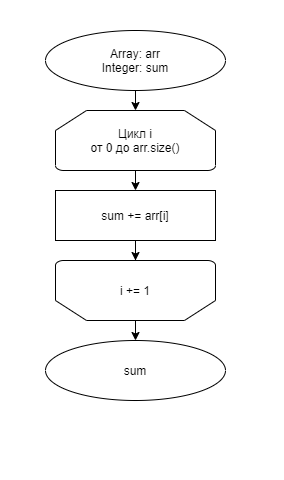
\includegraphics[scale=0.8]{sum_scheme}}
	\caption{Схема алгоритма поиска суммы всех элементов}
\end{figure}

\section{Алгоритм решения задачи без конвейера}

Используемые типы и структуры данных включают в себя:
\begin{enumerate}
	\item integer, целое число - используется для хранения индексов массива, размера массива;
	\item array, массив целых чисел - используется для хранения серии целых чисел.
\end{enumerate}

\newpage

\begin{figure}[ph!]
	\center{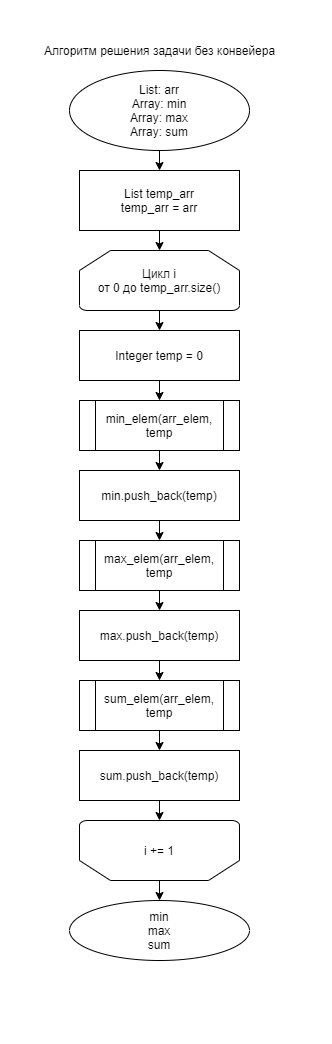
\includegraphics[scale=0.8]{alg_scheme}}
	\caption{Схема алгоритма решения задачи без конвейера}
\end{figure}

\section{Алгоритм решения задачи с конвейером}

Используемые типы и структуры данных включают в себя:
\begin{enumerate}
	\item integer, целое число - используется для хранения индексов массива, размера массива;
	\item array, массив целых чисел - используется для хранения серии целых чисел;
	\item matrix, массив массивов целых числел - представление матрицы в программе;
	\item vector, вектор - вид связного списка, позволяющий осуществять доступ к элементам по индексу.
\end{enumerate}

\newpage

\begin{figure}[ph!]
	\center{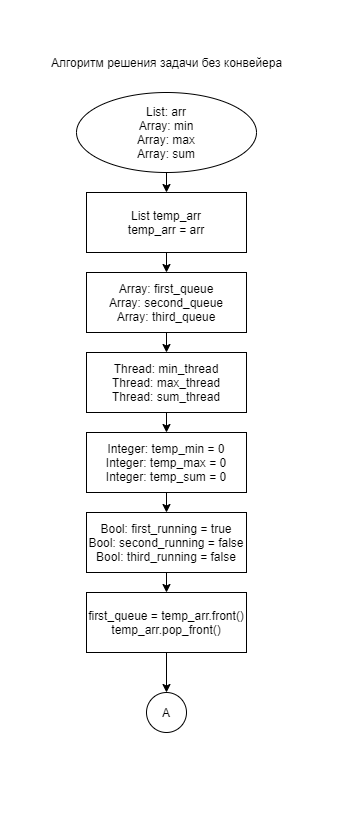
\includegraphics[scale=0.8]{conv_scheme_1}}
	\caption{Схема алгоритма решения задачи без конвейера часть 1}
\end{figure}

\newpage

\begin{figure}[ph!]
	\center{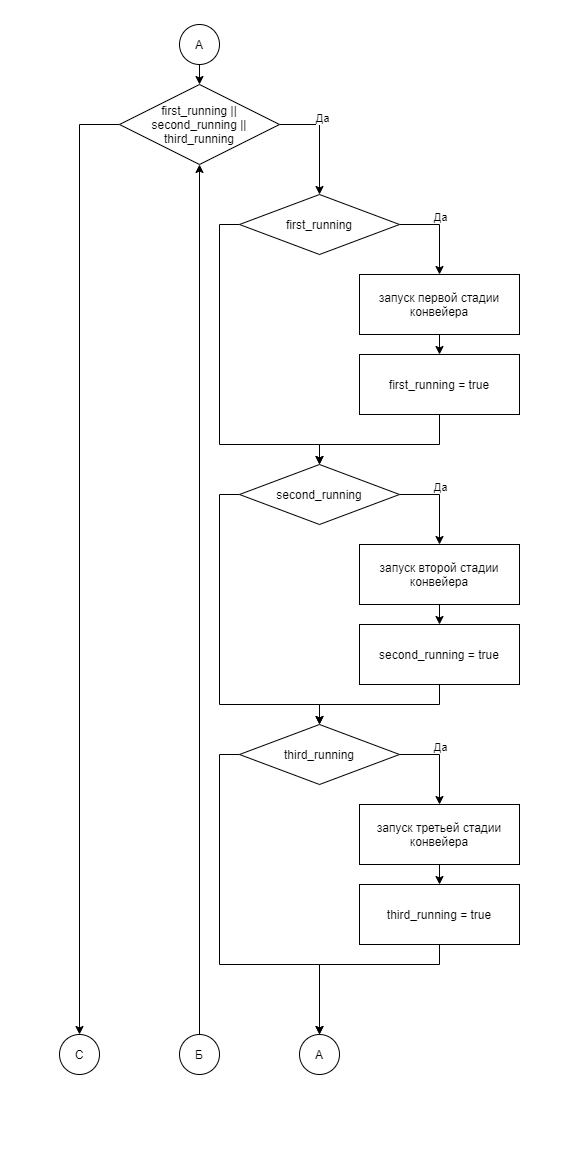
\includegraphics[scale=0.8]{conv_scheme_2}}
	\caption{Схема алгоритма решения задачи без конвейера часть 2}
\end{figure}

\newpage

\begin{figure}[ph!]
	\center{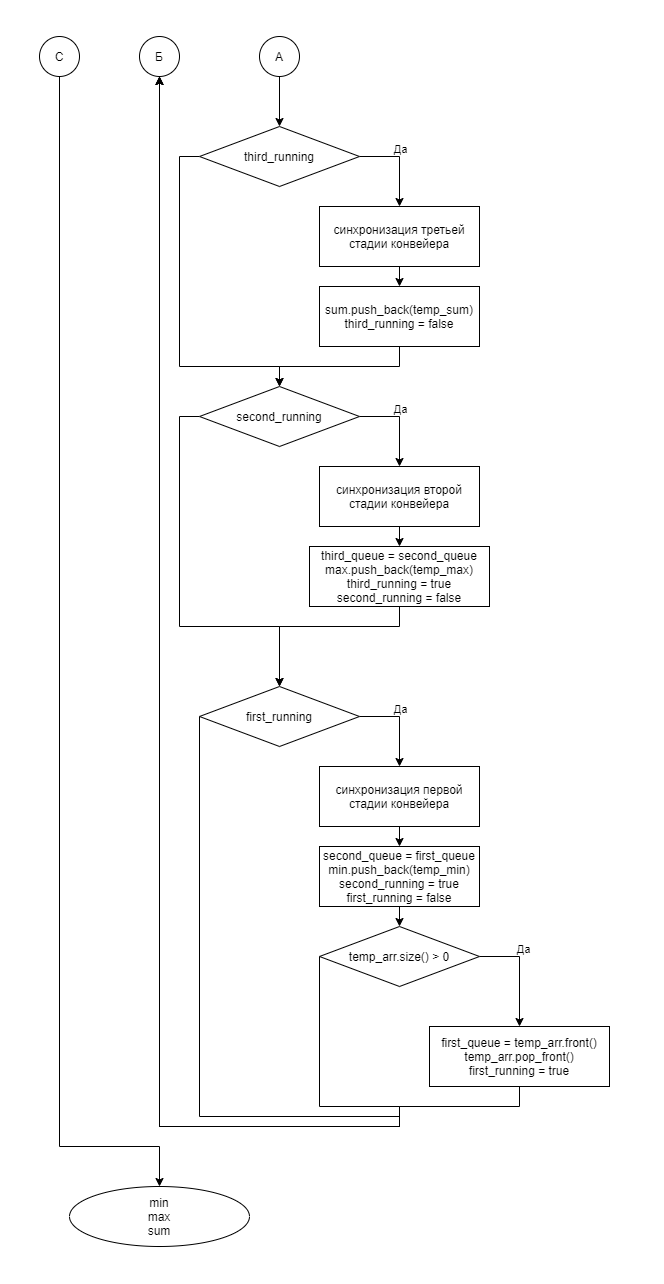
\includegraphics[scale=0.8]{conv_scheme_3}}
	\caption{Схема алгоритма решения задачи без конвейера часть 3}
\end{figure}

\newpage

\section{Функциональная схема ПО}
На изображении ниже представлена функиональная схема разрабатываемого ПО. На вход подаётся массив, заполненный целыми числами и при помощи алгоритмов, реализованных на языке С++ мы получаем в результате работы минимум, максимум и сумму всех элементов.

\begin{figure}[ph!]
	\center{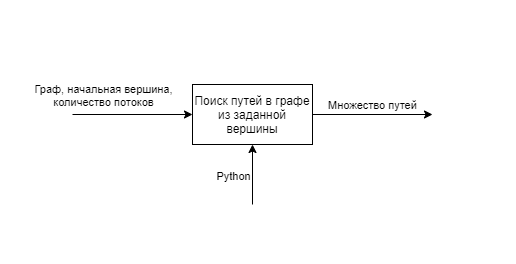
\includegraphics[scale=1.0]{func_scheme}}
	\caption{IDEF0 диаграмма разрабатываемой программы}
\end{figure}

\section{Вывод}
В данном разделе были рассмотрены схемы алгоритмов для поиска максимума, минимума, суммы всех элементов и алгоритмы решения задачи без и с конвейером. Были определены тесты для каждого алгоритма, были описаны типы и структуры данных, использующихся в алгоритмах. Также была приведена функциональная схема разрабатываемого ПО.

\chapter{Технологический раздел}

В данном разделе будут рассмотрены подробности реализации описаных выше алгоритмов. Также будут обоснованы выбор языка программирования для реализации, выбор библиотек для проведения экспериментов и представлены важные фрагменты кода написанной в рамках работы программы.

\section{Выбор языка программирования}

В качестве языка программирования для реализации данной лабораторной работы использовался язык программирования C++ поскольку в данном языке есть стандартная библиотека thread в которой реализованы основные методы для работы с потоками. В качестве среды разработки использовалась Microsoft Visual Studio 2019 по причине того, что данная среда имеет встроенные средства отладки и анализа программ.

\section{Сведения о модулях программы}

Реализованное ПО состоит из трёх модулей:
\begin{enumerate}
	\item conveyor - в данном модуле реализованы алгоритмы;
	\item lab\_5 - основной файл программы, где находится точка входа;
	\item tests - реализация тестов алгоритма;
	\item time - реализация замеров времени работы программы.
\end{enumerate}

\section{Реализация алгоритмов}

\begin{lstlisting}[label=some-code-1,caption=Реализация алгоритма поиска минимума]
void min_elem(std::vector<int> arr, int &min)
{
	min = arr[0];
	for (int i = 0; i < arr.size(); i++)
	{
		if (min > arr[i])
			min = arr[i];
	}
}
\end{lstlisting}

\begin{lstlisting}[label=some-code-2,caption=Реализация алгоритма поиска максимума]
void max_elem(std::vector<int> arr, int& max)
{
	max = arr[0];
	for (int i = 0; i < arr.size(); i++)
	{
		if (max < arr[i])
			max = arr[i];
	}
}
\end{lstlisting}

\begin{lstlisting}[label=some-code-3,caption=Реализация алгоритма поиска суммы всех элементов]
void sum_elem(std::vector<int> arr, int& sum)
{
	sum = 0;
	for (int i = 0; i < arr.size(); i++)
	{
		sum += arr[i];
	}
}

\end{lstlisting}

\begin{lstlisting}[label=some-code-4,caption=Реализация алгоритма без конвейера]
void conveyor::count_arr(std::list<std::vector<int>>& arr, std::vector<int>& min, std::vector<int>& max, std::vector<int>& sum)
{
	std::list<std::vector<int>> temp_arr;
	temp_arr = arr;
	for (auto& arr_elem : temp_arr)
	{
		int temp = 0;
		min_elem(arr_elem, temp);
		min.push_back(temp);
		max_elem(arr_elem, temp);
		max.push_back(temp);
		sum_elem(arr_elem, temp);
		sum.push_back(temp);
	}
}
\end{lstlisting}

\begin{lstlisting}[label=some-code-5,caption=Реализация алгоритма с конвейером]
void conveyor::count_arr_conv(std::list<std::vector<int>>& arr, std::vector<int>& min, std::vector<int>& max, std::vector<int>& sum)
{
	std::vector<int> first_queue;
	std::vector<int> second_queue;
	std::vector<int> third_queue;

	std::list<std::vector<int>> temp_arr;
	temp_arr = arr;

	std::thread min_thread;
	std::thread max_thread;
	std::thread sum_thread;

	int temp_min = 0;
	int temp_max = 0;
	int temp_sum = 0;

	bool first_running = true;
	bool second_running = false;
	bool third_running = false;

	first_queue = temp_arr.front();
	temp_arr.pop_front();

	while (first_running || second_running || third_running)
	{
		if (first_running)
		{
			min_thread = std::thread(min_elem, first_queue, std::ref(temp_min));
			first_running = true;
		}

		if (second_running)
		{
			max_thread = std::thread(max_elem, second_queue, std::ref(temp_max));
			second_running = true;
		}

		if (third_running)
		{
			sum_thread = std::thread(sum_elem, third_queue, std::ref(temp_sum));
			third_running = true;
		}

		if (third_running)
		{
			sum_thread.join();
			sum.push_back(temp_sum);
			third_running = false;
		}

		if (second_running)
		{
			max_thread.join();
			third_queue = second_queue;
			max.push_back(temp_max);
			third_running = true;
			second_running = false;
		}

		if (first_running)
		{
			min_thread.join();
			second_queue = first_queue;
			min.push_back(temp_min);
			second_running = true;
			first_running = false;
			if (temp_arr.size() > 0)
			{
				first_queue = temp_arr.front();
				temp_arr.pop_front();
				first_running = true;
			}
		}
	}
}
\end{lstlisting}

\section{Реализация тестирования алгоритмов}

Для тестирования алгоритмов было реализованы следующие тесты:
\begin{enumerate}
	\item тест на массивах, заполненных заранее известными значениями;
\end{enumerate}

\begin{lstlisting}[label=some-code-7,caption=Реализация тестов]      
void test()
{
	conveyor conv;
	std::list<std::vector<int>> arrs = { {1, 3, 4, -5}, {2, 4, 1, 4}, {1, 5, 2, 1}, {1, 3, 4, 5} };
	std::vector<int> min;
	std::vector<int> max;
	std::vector<int> sum;

	std::vector<int> min_true = { -5, 1, 1, 1 };
	std::vector<int> max_true = { 4, 4, 5, 5 };
	std::vector<int> sum_true = { 3, 11, 9, 13 };

	conv.count_arr(arrs, min, max, sum);

	std::cout << "Without conveyor result:" << std::endl;
	std::cout << "Minimun correct: " << (min == min_true) << std::endl;
	std::cout << "Maximun correct: " << (max == max_true) << std::endl;
	std::cout << "Sum correct: " << (sum == sum_true) << std::endl;

	max.clear();
	min.clear();
	sum.clear();
	conv.count_arr_conv(arrs, min, max, sum);

	std::cout << "With conveyor result:" << std::endl;
	std::cout << "Minimun correct: " << (min == min_true) << std::endl;
	std::cout << "Maximun correct: " << (max == max_true) << std::endl;
	std::cout << "Sum correct: " << (sum == sum_true) << std::endl;
}
\end{lstlisting}

\section{Вывод}
В данной разделе были представлены реализации алгоритма свёртки и параллельного алгоритма свёртки и показана реализация модуля тестирования реализованных алгоритмов.

\chapter{Экспериментальный раздел}

В данном разделе будут измерены временные характеристики алгоритмов свёртки и сделаны выводы об эффективности применения параллельного программирования для улучшения временных показателей данного алгоритма.

\section{Технические характеристики}
\begin{itemize}
	\item Операционная система - Windows 10, 64-bit;
	\item Оперативная память - 16 GiB;
	\item Процессор - Intel(R) Core(TM) i7-9750H CPU @ 2.60GHz 2.59 GHz, 6 ядер, 12 потоков.
\end{itemize}

\section{Результаты экспериментов}

\begin{table}[ph!]
  \begin{center}
    \captionsetup{justification=raggedright}
    \caption{Время работы алгоритмов часть 1}
    \label{tab:workcost_classic}
    \begin{tabular}{c|c|c}
      \textbf{Размерность} & \textbf{Без конвейера}  & \textbf{С конвейером} \\
      \hline
		10000 & 14410730 & 36757790\\
		20000 & 29048790 & 65201110\\   
		30000 & 41677490 & 66076070\\   
		40000 & 53177230 & 71010880\\   
		50000 & 65735330 & 75928700\\   
		60000 & 79101550 & 86291220\\   
		70000 & 92885460 & 99540600\\   
		80000 & 105098080 & 107917840\\ 
		90000 & 118854190 & 110939920\\ 
		100000 & 135586310 & 131559980\\
		110000 & 146946320 & 140116700\\
		120000 & 160452060 & 140567430\\
		130000 & 175246470 & 147778200\\
		140000 & 192886470 & 164722970\\
		150000 & 222497510 & 179168950\\
		160000 & 230255670 & 182251830\\
		170000 & 240874730 & 195043000\\
		180000 & 247061340 & 201011500\\
		190000 & 257129200 & 207278030\\
		200000 & 268234690 & 215100080\\
		210000 & 284637150 & 229495320\\
		220000 & 297554680 & 233842900\\
		230000 & 311475670 & 244595200\\
		240000 & 389308390 & 293369750\\
		250000 & 351293580 & 272306600\\
    \end{tabular}
  \end{center}
\end{table}

\begin{table}[ph!]
  \begin{center}
    \captionsetup{justification=raggedright}
     \caption{Время работы алгоритмов часть 2}
    \label{tab:workcost_classic}
    \begin{tabular}{c|c|c}
      \textbf{Размерность} & \textbf{Без конвейера}  & \textbf{С конвейером} \\
      \hline	
		260000 & 356309320 & 274189950\\
		270000 & 372085030 & 279380220\\
		280000 & 381061510 & 286817280\\
		290000 & 391780530 & 290586790\\
		300000 & 407649700 & 302525900\\
		310000 & 416702090 & 309778420\\
		320000 & 431093340 & 315700850\\
		330000 & 451243070 & 334894650\\
		340000 & 464012590 & 342740610\\
		350000 & 471855680 & 344893820\\
		360000 & 489654290 & 362364270\\
		370000 & 494999030 & 362130930\\
		380000 & 512794090 & 379268490\\
		390000 & 533304620 & 391316500\\
		400000 & 545626940 & 402669500\\
		410000 & 554232820 & 403925530\\
		420000 & 564171810 & 409611750\\
		430000 & 581163270 & 422192700\\
		440000 & 596754290 & 431110550\\
		450000 & 602919380 & 433952520\\
		460000 & 630570110 & 453187860\\
		470000 & 634635850 & 459071680\\
		480000 & 656107760 & 481584640\\
		490000 & 661004140 & 479517890\\
		500000 & 702121310 & 504461530\\
    \end{tabular}
  \end{center}
\end{table}

\begin{table}[ph!]
  \begin{center}
    \captionsetup{justification=raggedright}
     \caption{Лог работы программы}
    \label{tab:workcost_classic}
    \begin{tabular}{c|c|c|c}
      \textbf{Номер конвейера} & \textbf{Номер заявки}  & \textbf{Время начала}  & \textbf{Время конца}\\
      \hline	
		1 & 1 & 2900 & 20141800\\
		2 & 1 & 30015400 & 35058300\\
		1 & 2 & 29820600 & 42582600\\
		3 & 1 & 51763000 & 59150500\\
		2 & 2 & 49758300 & 65423100\\
		1 & 3 & 49545000 & 71573200\\
		3 & 2 & 82941800 & 98629500\\
		2 & 3 & 79447700 & 104511900\\
		1 & 4 & 79232900 & 108953300\\
		3 & 3 & 111954600 & 114019500\\
		2 & 4 & 111278500 & 115988000\\
		1 & 5 & 111163000 & 118624000\\
		3 & 4 & 122693000 & 124279400\\
		2 & 5 & 120866100 & 126324900\\
		1 & 6 & 120666900 & 127200300\\
		3 & 5 & 128527000 & 130745200\\
		2 & 6 & 127979500 & 131521400\\
		1 & 7 & 127898000 & 132199000\\
		3 & 6 & 133430100 & 135606000\\
		2 & 7 & 132917000 & 136353900\\
		1 & 8 & 132869900 & 138477000\\
		3 & 7 & 140910700 & 143018500\\
		2 & 8 & 140807800 & 144370600\\
		3 & 8 & 145263500 & 146321500\\
    \end{tabular}
  \end{center}
\end{table}


\newpage

\begin{figure}[ph!]
	\center{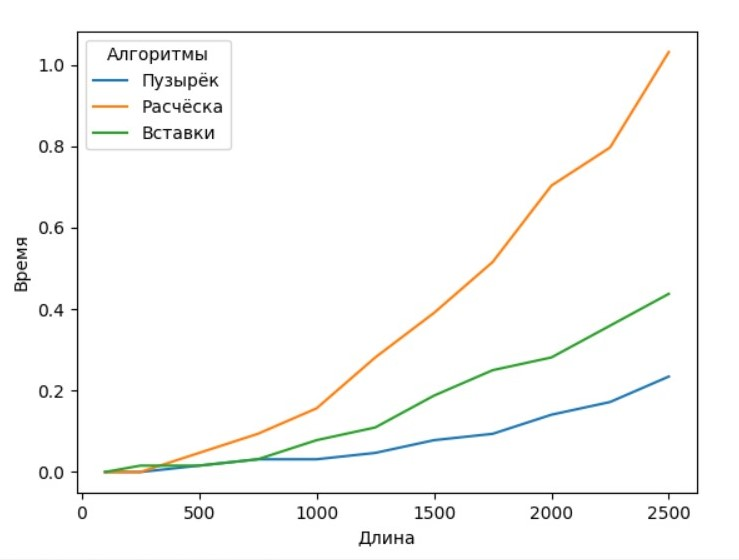
\includegraphics[scale=0.6]{res_graph}}
	\caption{График зависимости времени работы от размерности массивов}
\end{figure}

\section{Вывод}
В результате эксперимента было получено, что на квадратных массивах размерами от 10000 до 500000 использование конвейера позволяет добиться ускорения в 1.39 раз по времени выполнения. В результате можно сделать вывод о том, что использование ковейерного программированния позволяет ускорить обработку больших задач.